%%%%%%%%%%%%%%%%%%%%%%%%%%%%%%%%%%%%%%%%%%%%%%%%%%%%%%%%%%%%
%% PLANTILLA LATEX PARA PRESENTACION DE TRABAJOS DE GRADO %%
%% Formato:                                               %%
%%         letterpaper: tamaño carta                      %%
%%         12pt       : letra de tamaño 12                %%
%%                    : espaciado simple                  %%
%% Preparado: Oscar Danilo Montoya						  %%
%%%%%%%%%%%%%%%%%%%%%%%%%%%%%%%%%%%%%%%%%%%%%%%%%%%%%%%%%%%% 
\documentclass[letterpaper,12pt, oneside]{book}
\usepackage{TesisUTB}
\usepackage{hyperref}
\usepackage{graphicx}
\graphicspath{ {img/} }
\usepackage[utf8]{inputenc}
\usepackage{listings,xcolor}
\usepackage{inconsolata}

\definecolor{dkgreen}{rgb}{0,.6,0}
\definecolor{dkblue}{rgb}{0,0,.6}
\definecolor{dkyellow}{cmyk}{0,0,.8,.3}

\lstset{
  language        = php,
  basicstyle      = \small\ttfamily,
  keywordstyle    = \color{dkblue},
  stringstyle     = \color{red},
  identifierstyle = \color{dkgreen},
  commentstyle    = \color{gray},
  emph            =[1]{php},
  emphstyle       =[1]\color{black},
  emph            =[2]{if,and,or,else},
  emphstyle       =[2]\color{dkyellow},
  keywords    ={__halt_compiler,    abstract,   and,    array,
                    as, break,  callable,   case,   catch,  class,
                    clone,  const,  continue,   declare,    default,
                    die,    do, echo,   else,   elseif,
                    empty,  enddeclare, endfor, endforeach, endif,
                    endswitch,  endwhile,   eval,   exit,   extends,
                    final,  finally,    for,    foreach,    function,
                    global, goto, if,   implements, include,
                    include_once,   instanceof, insteadof,
                    interface,  isset, list,    namespace,
                    new,    or, print, private, protected,  public,
                    require,    require_once, return,   static,
                    switch, throw,  trait, try, unset, use, var,
                    while,  xor,    yield,
  },
 }


%%%%%%%%%%%%%%%%%%%%% DATOS DEL AUTOR %%%%%%%%%%%%%%%%%%%%%%
\def\AUTOR{\textbf{Miguel Isaza}}
\def\TITULO{Aplicación de metodologías de mantenimiento ágil al servicio ALTEM en la UTB}
%% CUAL METODOLOGÍA??? miguel


\def\DIRECTOR{\textbf{Jairo Enrique Serrano Castañeda}, M.Sc. \\ Universidad Tecnológica de Bolívar}

\def\FECHA{\today}

%%%%%%%%%%%%%%%%%%%%%%%%%%%%%%%%%%%%%%%%%%%%%%%%%%%%%%%%%%%%

\setcounter{secnumdepth}{3}
\setcounter{tocdepth}{3}

% quitar el 0.
\renewcommand\thesection{\arabic{section}}
%\renewcommand*{\bibfont}{\footnotesize}

% tabla de contenidos como seccion
\makeatletter
\renewcommand\tableofcontents{
	\section*{{Tabla de contenidos} %linea importante
		\@mkboth{
			\MakeUppercase\contentsname}{\MakeUppercase\contentsname}}
	\@starttoc{toc}
}
\makeatother

% bibliografia como seccion
\makeatletter
\renewenvironment{thebibliography}[1]{
	\section*{Referencias} %linea importante
	\@mkboth{\MakeUppercase\bibname}{\MakeUppercase\bibname}
	\list{\@biblabel{\@arabic\c@enumiv}}
	{\settowidth\labelwidth{\@biblabel{#1}}
		\leftmargin\labelwidth
		\advance\leftmargin\labelsep
		\@openbib@code
		\usecounter{enumiv}
		\let\p@enumiv\@empty
		\renewcommand\theenumiv{\@arabic\c@enumiv}}
	\sloppy
	\clubpenalty4000
	\@clubpenalty \clubpenalty
	\widowpenalty4000
	\sfcode`\.\@m}
{\def\@noitemerr
	{\@latex@warning{Empty `thebibliography' environment}}
	\endlist}
\makeatother

% aqui definimos el encabezado
%\lhead[\thepage/\pageref{LastPage}]{}
%\chead[Informe]{Proyecto de grado}
%\rhead[]{\thepage/\pageref{LastPage}}
\renewcommand{\headrulewidth}{0.5pt}

% aqui definimos el pie de pagina
\lfoot[]{Miguel Isaza - UTB}
\cfoot[\today]{\today}
\rfoot[]{UTB}
\renewcommand{\footrulewidth}{0.5pt}

\pagestyle{fancy}

% margenes
\setlength{\oddsidemargin}{10mm}
\setlength{\evensidemargin}{10mm}

\raggedbottom

\begin{document}
\frontmatter
\renewcommand{\maketitle}{

%------------- Portada ---------------------------

\begin{titlepage}

\begin{center}

\large
\textbf{\TITULO}

\vfill
\vfill
\vfill
\vfill
\normalsize
\AUTOR \\
\vspace{1cm}
Trabajo de grado sometido como requisito parcial\\
para optar por el título de \\
\textbf{Ingeniero(a) de Sistemas} \\

\vfill
\vfill
%Director\\
%\DIRECTOR\\
\vfill

%\
%Co-Directores\\
%\CODIRECTOR\\
\vfill


\begin{figure}[b]
\centering

\includegraphics[scale = 0.5]{UTB.png}
\end{figure}

\FECHA \\
\UTP \\
Programa de Ingeniería de Sistemas y Computación\\


\end{center}

\end{titlepage}
\normalsize

\newpage
\thispagestyle{empty}

\begin{flushright}
\vfill
\textbf{\Large{Solicitud de evaluaci\'on}} \\
\vfill
\textit{Trabajo de grado sometido como requisito parcial para iniciar el proceso de investigación conducente al proyecto de grado en la Universidad Tecnológica de Bol\'ivar}
%\rule{8cm}{1pt} \\
%\rule{8cm}{1pt} \\
%\rule{8cm}{1pt} \\
\vspace{2cm}

\rule{8cm}{1pt} \\


\AUTOR .\\Universidad Tecnológica de Bolívar. Estudiante(s) \\
\vspace{2cm}

Revisado por: \\
\vspace{2cm}

\DIRECTOR . Director \\
\vspace{-2cm}
\rule{8cm}{1pt} \\
%\rule{8cm}{1pt}\\
%Jurado \\

\vfill
Cartagena D. T. y C., \FECHA \\
\end{flushright}
\normalsize

}

\maketitle
\chapter*{Dedicatoria} 
\chapter*{Agradecimientos} 
\chapter*{Resumen} 

\chapter{Abstract}

This work consists in the application of agile methodologies to ALTEM, which is a software project of the Universidad Tecnológica de Bolívar proposed by the Department of University Welfare due to the need to control the student population that meets certain risk factors, this project would help the psycologists of University Welfare to prevent student desertion.

The main function of this software is to identify active students who present a risk condition. When a student is identified, the software triggers an alert for this student in order to be intervened by the student counseling team and track its progress in a logbook. 

The software is capable of generating a list of students who meet these risk conditions, when you access one of these students in details, the software shows a timeline in which you can add information of actions and strategies that have been applied to the student since the alert was triggered until it leaves the risk situation. 

This software was initially developed by Hernando Ariza during 2016 and presented as his degree work. 

During the following year, University Welfare staff began testing this software, in order to get feedback and decide if the project was sustainable enough to continue its funding. 

At the end of that year, it was concluded that the software could meet the objectives for which it was created, but had certain shortcomings at the level of functionality, user experience and requirements.

Consequently, at the beginning of 2018 Miguel Isaza decided to continue with the maintenance and development of this project, which now presented new functional requirements and required bug fixes.

A work plan was designed which consisted of developing the new functionalities and improving the problems presented by the software at that time, performing QA processes so it can enter a in a trial period again by the University Welfare staff to receive new feedback. 

\tableofcontents
\addcontentsline{toc}{chapter}{Índice general}

\renewcommand{\listtablename}{Índice de tablas}
\listoftables
\addcontentsline{toc}{chapter}{Índice de tablas}
\listoffigures
\addcontentsline{toc}{chapter}{Índice de figuras}
\cleardoublepage
\mainmatter

%%%%%%%%%%%%%%%%%%%%%%%%%%%%%%%%%%%%%%%%%%%%%%%%%%%%%%%%%%%%%%%%
%%%%%%%%%%%%%%%%%%%%%%%%%%%%%%%%%%%%%%%%%%%%%%%%%%%%%%%%%%%%%%%%%%%%%
%%%%%%%%%%%%%%%%%%%%%%%%%%%%%%%%%%%%%%%%%%%%%%%%%%%%%%%%%%%%%%%%%%%%%


%%%%%%%%%%%%%%%%%%%%%%%%%%%%%%%%%%%%%%%%%%%%%%%%%%%%%%%%%%%%%%%%%%%%%
%%%%%%%%%%%%%%%%%%%%%%%%%%%%%%%%%%%%%%%%%%%%%%%%%%%%%%%%%%%%%%%%%%%%%
\chapter{Introducci\'on}
ALTEM es una aplicación de software cuya función principal es servir de apoyo a la gestión de Bienestar Estudiantil en lo referente al seguimiento de estudiantes en situaciones de interés, desde el momento de su inscripción, entrevista y posterior ingreso a clases. Las situaciones de interés mencionadas corresponden a eventos como la prueba académica, o condiciones de vulnerabilidad relacionadas al entorno socio- económico del estudiante, entre otras.

ALTEM se concibe entonces como una herramienta que le debe permitir a Bienestar Estudiantil identificar a los estudiantes que se encuentran en alguna de estas situaciones de interés, para iniciar los procedimientos del caso. Adicionalmente, el sistema debe permitir contar con un registro de las acciones e intervenciones que se han llevado a cabo sobre la situación de los estudiantes identificados. La meta final es evitar la posible deserción estudiantil.

\section{Justificación}
Toda institución académica llega a al punto de quiebre en el cual necesita un departamento de bienestar estudiantil, el cual se encarga de vigilar la calidad académica de los estudiantes. Cuando el volumen de estudiantes es muy grande, surge la necesidad de implementar sistemas de información que faciliten a los consejeros estudiantiles llevar un control de estos estudiantes. 

Al ser una necesidad inminente, se han venido implementando sistemas de información que nos brindan soluciones para esta problemática, como lo son SATD de Foris, los cuales se venden y distribuyen como un producto comercial.

ALTEM surge como una alternativa a estos sistemas, cuyo valor agregado es su seguimiento en forma de bitácora, lo que hace que la experiencia de usuario sea considerablemente más agradable con respecto a sus iguales.

Durante el desarrollo de ALTEM, se introdujeron diversos patrones y diseños en la arquitectura del software que dificultaron la extensión de este al implementar nuevos requerimientos, además de la presencia de considerables fallas o bugs que complicaban la interacción con el usuario y en consecuencia afectaba negativamente la calidad general del software.

Este proyecto parte de la necesidad de aplicar las metodologías ágiles en un plan de extensión de la plataforma ALTEM, con el fin de mejorar falencias a nivel de funcionalidad y experiencia de usuario mencionadas anteriormente.

\section{Estado del arte}
 Debido al gran número de estudiantes que en las últimas décadas han accedido a la Educación Superior, se ha venido implementado de forma gradual en varios países, investigaciones y estrategias para aumentar la retención de estudiantes en este nivel\cite{garinsallan}

 En Latinoamérica la investigación ha sido más reciente, aunque ha adquirido en la última década un gran impulso.\cite{SATPaper}

\subsection{Productos Internacionales}

 \subsubsection{\textit{Frederick Community College}}
 Durante el año académico 2007-2008 se testeó un Sistema de Alertas Tempranas en ciertos cursos, procedimiento extendido a toda la Universidad una vez adquirida la infraestructura tecnológica para ello. La estrategia se basó en un sitio Web donde los docentes completaban un informe sobre el rendimiento del estudiante. Los profesores disponen de una lista electrónica para identificar y caracterizar los estudiantes que no están asistiendo y/o tienen bajas calificaciones. El sistema provee un formato automático que identifica el problema y hace recomendaciones para la provisión de intervenciones, usualmente sustentada en una entrevista entre el estudiante y su tutor. La información es compartida con el estudiante, siendo su caso asignado a un consejero académico \cite{chapellc} 
 Los resultados han sido positivos: desde el 2008, el porcentaje de casos exitosos ha subido de 52\% a 66\%.
 
  \subsubsection{\textit{Foris (SATD)}}
  Foris, empresa con presencia en Latinoamérica (7 países), se dedica al desarrollo de software para gestión académica universitaria. Uno de sus productos es el Sistema de Alerta Temprana de Deserción (SATD), plataforma que basándose en indicadores históricos de deserción, permite predecir la deserción de estudiantes. El análisis que hace el sistema, se basa en un enfoque cuantitativo y cualitativo con una metodología de predicción de la deserción. La Ilustración 1 muestra el flujo de
  esta metodología
  El enfoque cuantitativo se sustenta en modelos matemático/estadísticos y de minería de datos, que consideran, entre otras variables las calificaciones de los estudiantes, datos demográficos – contemplados está la definición de factores de riesgo para generar perfiles de alumnos desertores y elaborar planes de apoyo oportuno y específico para cada grupo de estudiantes.\cite{SATPaper}.
 

 \subsection{Productos Nacionales}
   \subsubsection{\textit{Universidad Tecnológica de Pereira}}
 En el caso de Colombia, un grupo de investigadores ha trabajado 9 años en la exploración de las causas de la deserción estudiantil la Universidad Tecnológica de Pereira y las maneras para contrarrestarlas, probando estrategias de intervención. Esto ha conducido al diseño de un modelo de SAT: en 6 años se disminuyó la deserción de 15 a 10\%. Además ha incentivado que el gobierno fortalezca los programas de fomento a la permanencia en varias IES. \cite{carvajal}
 
\subsection{Marco Teórico}
(en qué teorías me baso para desarollar el proyecto)
\subsection{Marco Conceptual}

(conceptos y palabras claves que se deben aclarar para que el lector sepa, todo referenciable)

(como recbií el proyecto y como lo redirecciono para concluirlo)

MVC 


\subsection{Marco Legal}
(Leyes colombianas de Habeas Data y proteccion de datos sensibles)
\subsection{Marco Ético}
(Compromiso por parte de los desarolladores del compromiso con los datos sensibles manejados en las bases de datos)
\section{Objetivos}

\subsection{Objetivo General}
Desarrollar un plan de mejoramiento de la aplicación ALTEM para reactivar su uso por parte de los consejeros académicos del departamento de Bienestar Universitario en la Universidad Tecnológica de Bolívar.

\subsection{Objetivos Específicos}
\begin{itemize}
    \item Actualizar el algoritmo de autenticación de usuarios (de LDAP a SAVIO)
    \item Conectar, consumir y sincronizar los datos académicos y estudiantiles de ALTEM con el nuevo sistema BANNER de forma automatizada.
    \item Hacer mejoras en las animaciones del Front-End
    \item Analizar las falencias en la experiencia de usuario y hacer mejoras en ese aspecto
    \item Resolver las fallas (bugs) presentes en la aplicación.
    \item Hacer refactorización de los módulos que presentan problemas de calidad de código y arquitectura.
    \item Implementar los nuevos requerimientos solicitados el personal de consejería académica
\end{itemize}
\chapter{Requerimientos}

\section{Requerimientos funcionales}

\begin{itemize}
 \item Autenticación de usuarios (Savio) (Moodle)
 \item Información del usuario (Savio)
  \begin{itemize}
         \item Foto
         \item Nombre completo
    \end{itemize}
 \item Visualización de horarios de clase (Banner)
 \item Visualización mapa UTB (Imagen sobre API google maps)
 \item Visualización de contactos
 \item Centro de notificaciones
     \begin{itemize}
         \item Savio
         \item Web
         \item Academia
    \end{itemize}
 \item Visualización de notas parciales (Banner)
 \item Visualización de cursos (Savio)
    \begin{itemize}
         \item Información del profesor
         \item Tareas pendientes
    \end{itemize}
\end{itemize}

\section{Requerimientos no funcionales}
 \begin{itemize}
         \item Aplicación móvil (Android y IOS)
         \item Rápida al hacer las consultas
         \item Liviana en el móvil 
         \item Visualmente atractiva
\end{itemize}


\chapter{Diseño y modelado}

\section{Arquitectura}
ALTEM es una aplicación web de Stack Completo la cual está compuesta por las siguientes tecnologías
\begin{itemize}
    \item Front-End: Javascript ES5 con AngularJS 1.6
    \item BackE-End: PHP 7.1 con Laravel.
    \item Bases de Datos: SQL por MySQL.
\end{itemize}

Su API también se comunica con otros sistemas que pertenecen a la universidad, tales como

\begin{itemize}
    \item LDAP (Actualmente Deprecado)
    \item SAVIO (Moodle)
    \item Banner (Oracle)
\end{itemize}

En la Figura 3.1 Se puede apreciar la Arquitectura de ALTEM y la relacion existente entre cada uno de los elementos del stack y las APIs externas. 

\begin{figure}[H]
    \centering
    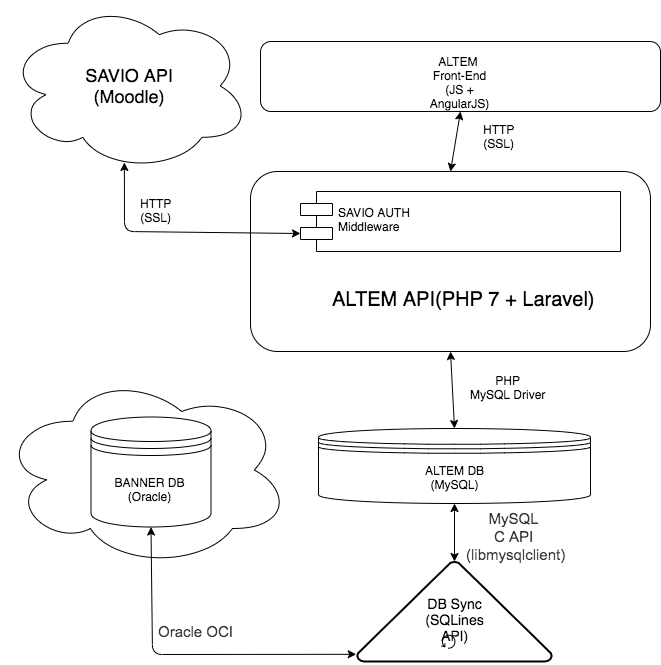
\includegraphics[width=0.7\textwidth]{img/ALTEM.png}
    \caption{Arquitectura de ALTEM}
\end{figure}

\subsection{Cliente (Front-End)}
Al ser una aplicacion web, ALTEM se consume desde el navegador, por medio de un Front-End creado en HTML5, CSS y JavaScript.

La capa de JavaScript está manejada por AngularJS 1.6, el cual nos facilita el desarrollo de las funcionalidades utilizando el patrón MVC el cual es un patrón de arquitectura de software, que separa los datos y la lógica de negocio de una aplicación de su representación, y el módulo encargado de gestionar los eventos y las comunicaciones.
MVC propone la construcción de tres componentes distintos que son el modelo, la vista y el controlador, es decir, por un lado define componentes para la representación de la información, y por otro lado para la interacción del usuario.\cite{trygve}

La aplicación web está compuesta por varios módulos, cada uno con sus modelos, vistas y controladores.

Los módulos son los siguientes:

\begin{itemize}
    \item Acción
    \item Estrategia
    \item Filtros
    \item Login
    \item Reportes
    \item Riesgos
    \item Tipos de Riesgos
    \item Usuarios
\end{itemize}

\subsubsection{Modelo}
Para el caso del cliente web, nuestro modelo equivale a todos los datos que vienen desde la API y que se solicitan por medio de peticiones HTTP. Estos datos se guardan en el localStorage y sessionStorage, y representan toda la información que el usuario puede ver a través de la vista en tiempo real.

Estas solicitudes a la API se encuentran organizadas en Servicios\cite{servicios} los cuales ejecutan llamadas a distintos endpoints\cite{endpoints}.

\begin{itemize}
    \item Acción
    \item Archivo Personal
    \item Criterio
    \item Estrategia
    \item Estudiante
    \item Filtro
    \item Intervención
    \item Login
    \item Observación
    \item Reporte
    \item Riesgo
    \item Tipo Riesgo
    \item Usuario
\end{itemize}

Estos servicios se comunican con el Back-End a trvés de la API de XMLHttpRequest(XHR) y utilizando métodos HTTP.

El Modelo es modificado por los Controladores, los cuales actualizan el estado de los datos dependiendo de las interacciones que tenga la aplicación con el usuario.
\subsubsection{Controlador}
Los controladores son funciones que disparan las instrucciones que modifican el Modelo, generalmente llamadas en la vista a través de eventos y en los servicios a través de Promesas.
En la aplicación web, todas las acciones (iniciar sesión, ver estudiantes, añadir estrategias, filtrar búsquedas, etc) disparan estos controladores, estos controladores se encuentran categorizados por los módulos mencionados en 1.1.

Las funciones principales de los controladores en la aplicación web son los siguientes:

\begin{itemize}
    \item Mutar el estado local de la aplicación.
    \item Hacer llamadas a los servicios.
    \item Actualizar la Vista.
\end{itemize}

Por lo general, las acciones ejecutadas en los controladores hacen que la vista se refresque.

\subsubsection{Vista}
La Vista se concibe como la capa presentacional de la aplicación web. Es la parte que interactúa con el usuario directamente y es la que se encarga de renderizar todos los datos del modelo en una manera que el usuario puede comprender fácilmente. 

Las vistas están hechas a través de plantillas HTML5 estilizadas con CSS, las cuales se renderizan de forma dinámica a medida que el modelo de la aplicación se actualice y se vayan ejecutando eventos que disparen los controladores.

La vista también se actualiza por medio de las directivas de AngularJS.

\subsection{Servidor (Back-End)}
El Back-End es el núcleo de ALTEM, consiste en una app Laravel y PHP7 en la que se encuentra toda la lógica del servidor.
Al igual que el Front-End, esta aplicación comparte la misma arquitectura MVC, pero orientada al lado del servidor.

También, se encarga de comunicarse con API's de terceros como BANNER y SAVIO, plataformas pertenecientes a los recursos tecnológicos de la Universidad Tecnológica de Bolívar para obtener datos esenciales para su funcionamiento, de los cuales hablaremos más adelante. 

\subsubsection{Modelo}
Para nuestro Back-End, el Modelo es una representación de la estructura de los datos y relaciones que se manejan  base de datos, en clases y objetos que comparten la misma estructura. Esto con el propósito de que se maneje una consistencia entre la base de datos y la API.

Para hacer esa integración posible, se utiliza una API llamada Eloquent, la cual nos permite construir y ejecutar consultas a la base de datos utilizando definiciones y métodos propios del lenguaje. Esto también se conoce como ORM.

Para cada tabla existente en la base de datos, existe un modelo correspondiente en el back-end el cual se representa mediante una Clase como lo muestra el siguiente ejemplo:

\begin{lstlisting}
namespace App\Models;

class Tabla extends Model
{
    protected $table = 'nombre_tabla';
    
    // columnas de la tabla
    protected $fillable = ['columna1', 'columna2', 'columna3'];

    //PK
    protected $primaryKey= "codigo";

    // Relaciones
    public function relacion1()
    {
        // Ejemplo 1:N
        return $this->belongsToMany('OtroModelo','FK','FK','FK');
    }

    public function relacion2(){
        // Ejemplo 1:1
        return $this->hasOne('OtroModelo','FK','FK');
    }
}
\end{lstlisting}

Esta clase extiende de Model, la cual es una clase implementada por Laravel para manejar las relaciones entre tablas. Esa clase posee varios metodos como los observados previamente.

\subsubsection{Controlador}
En el caso del Back-End, los controladores son clases que poseen los métodos que ejecutan la lógica de la aplicación y hacen los cambios en la base de datos al llamar a los Modelos

Una clase controladora se compone de la siguiente manera:

\begin{lstlisting}
namespace App\Http\Controllers;

// importamos Modelo relacionado con el controlador
use \Models\Tabla;

class Acciones extends Controller
{
    public function __construct()
    {
        // Usamos middlewares necesarios
        $this->middleware('cors');
    }

    public function obtener_todos()
    {
       $datos = Tabla::all();
        return response()->json($datos);
    }
    
     public function obtener_por_codigo($codigo)
    {
        $datos_codigo = Tabla::find($codigo);
        return response()->json($datos_codigo);
    }
    
      public function eliminar_por_codigo($id)
    {
        $datos_de_id = Tabla::find($id);
        $datos_de_id->delete();
        return response()->json(["mensaje" => "Eliminado con Exito"]);
    }
}
\end{lstlisting}

En este ejemplo, podemos observar como la la clase Acciones posee varios métodos que llaman a Modelo y ejecutan varios métodos sobre este. Estos metodos representan consultas SQL que modifican los datos en la base de datos.
Al final de las instrucciones, se retornan los datos solicitados o el mensaje por medio de JSON.

\subsubsection{Vista}
Al ser una API, en este caso la vista no representa ninguna capa de interacción con el usuario sino más bien un conjunto de rutas o endpoints los cuales son consultados mediante HTTP y que son el puente entre el Back-End y el Front-End.

\subsection{Bases de Datos}
Las bases de datos de ALTEM son de tipo SQL, ejecutadas en el motor MySQL X, todas las consultas son manejadas por el ORM del Back-End

Al ser una base de datos Relacional, fue necesario establecer un conjunto de relaciones entre tablas para mantener la consistencia y confiabilidad en los datos utilizados en la aplicación, como se aprecia en la Figura 3.2.

\begin{figure}[H]
    \centering
    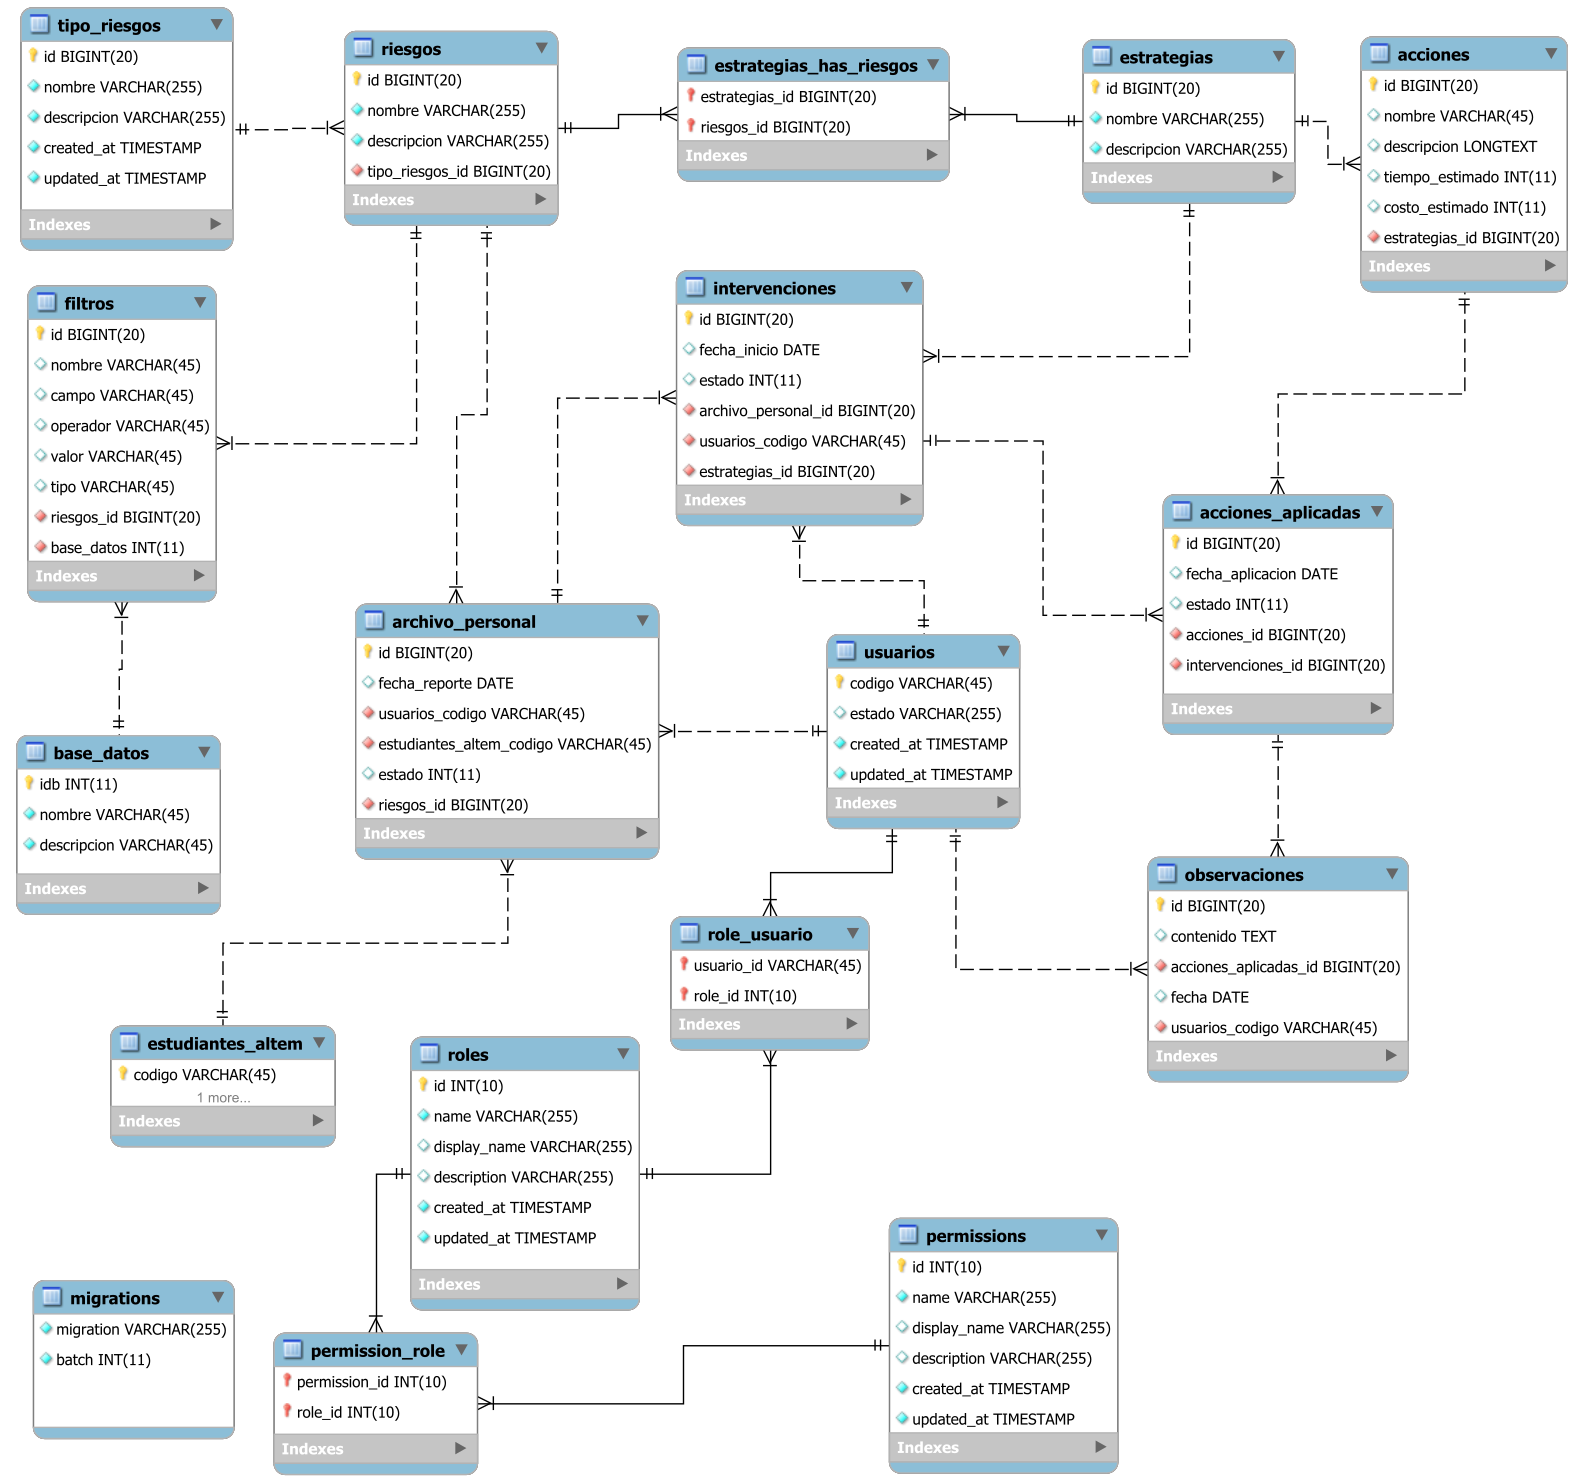
\includegraphics[width=1\textwidth]{img/EER.png}
    \caption{Relación de entidades en la base de datos de ALTEM.}
\end{figure}

\subsection{Herramientas}
    \begin{itemize}
         \item JavaScript
         \item React native
    \end{itemize}
 \subsection{Modelos de desarrollo}
     KANVAN

\section{Plan de trabajo}

\subsection{Prioridad A}
\begin{itemize}
 \item Autenticación de usuarios (Savio) (Moodle)
 \item Información del usuario (Savio)
    \begin{itemize}
         \item ID
         \item Foto
         \item Nombre completo
         \item ...
    \end{itemize}
 \item Visualización de contactos (Universidad)
  \begin{itemize}
         \item Web
         \item Twiter, facebook...
         \item Números telefónicos
         \item ...
    \end{itemize}
 \item Visualización de cursos (Savio)
   \begin{itemize}
         \item Información del profesor
         \item Tareas pendientes
         \item ...
    \end{itemize}
\end{itemize}


\subsection{Prioridad B}
\begin{itemize}
 \item Visualización de notas parciales (Banner)
 \item Visualización de horarios de clase (Banner)
 \begin{itemize}
        \item Nombre del curso
        \item Hora
        \item Lugar
         \item ...
    \end{itemize}
\end{itemize}

\subsection{Prioridad C}
\begin{itemize}
 \item Visualización mapa UTB (Imagen sobre API google maps)
 \item Centro de notificaciones
     \begin{itemize}
         \item Savio
         \item Web
         \item Academia
    \end{itemize}
\end{itemize}
\chapter{Integración y fuentes de datos}
\chapter{Implementación y despliegue}
Al ser de una arquitectura modular, podemos automatizar el proceso de implementación y despliegue de la aplicación en los servidores, por medio de contenedores como Docker


\chapter{Pruebas y resultados}
\chapter{Conclusiones}
\section{Recepción del Proyecto}
ALTEM es un proyecto de la universidad Tecnológica de Bolívar que ha facilitado el proceso de atención a los estudiantes por parte de los consejeros del departamento de bienestar universitario, los cuales determinan que el proyecto ha sido satisfactorio y que el software se encuentra en un punto de usabilidad plena con buenas expectativas hacia el futuro. 

Se considera que ALTEM debe seguir siendo desarrollado ya que los costos de desarrollo de este proyecto son considerablemente inferiores al hecho de adquirir un nuevo producto que cumpla con los mismos requerimientos. 
Los consejeros se encuentran motivados y determinados a seguir utilizando la plataforma como herramienta principal para el seguimiento de sus estudiantes, con toda la disposición de realizar un nuevo plan de trabajo con requerimientos nuevos los cuales harían la aplicación aún más confiable y de usabilidad más integral, no solo para ellos sino para otros departamentos de la Universidad Tecnológica de Bolívar. 

En términos generales, el recibimiento por parte del departamento de Bienestar fue positivo y consideran totalmente viable la continuidad en la inversión del proyecto.

\section{Conclusiones del Autor}
El autor de este trabajo como desarrollador de software considera que la aplicación cuenta con una arquitectura fácil de mantener, pero existen componentes dentro de esta arquitectura que tienen dependencias las cuales se encuentran en estado de depreciación o están cerca de estarlo, por lo cual se recomienda que se haga una actualización del código fuente para que este pueda ser más fácil de mantener y tenga mayor apoyo por parte de la comunidad Open-Source en la que están basadas varias de sus dependencias.
Una de esas dependencias es el Framework sobre el cual se basa la API. El cual es una versión de Laravel muy cerca de quedar depreciada. Se considera que la mejor solución es migrar esa API a la nueva implementación ligera de Laravel conocida como Lumen, ya que tiene una orientación mas acertada al tipo de API que se desarrolló para este proyecto.



%%%%%%%%%%%%%%%%%%%%%%%%%%%%%%%%%%%%%%%%%%%%%%%%%%%%%%%%%%%%%%%%%%%%%
%%%%%%%%%%%%%%%%%%%%%%%%%%%%%%%%%%%%%%%%%%%%%%%%%%%%%%%%%%%%%%%%%%%%%
\newpage
%%%%%%%%%%%%%%%%%%%%%% - BIBLIOGRAFÍA - %%%%%%%%%%%%%%%%%%%%%%%%


\bibliographystyle{IEEEtran}
\begin{thebibliography}{}


\bibitem{garinsallan}
GAIRÍN SALLÁN, J.
\textit{Los sistemas de acceso, normativa de permanencia y estrategias de tutoría y retención de estudiantes de Educación Superior.} Madrid: Wolters Kluwer, 2015.
\bibitem{chapellc}
CHAPPELL, C. 
\textit{Early alert’ systems send students warnings, advice. 2010.} Disponible en: \url{http://www.ccdaily.com/Pages/Campus-Issues/Early-alert- systems-send-students-warnings-advice.aspx}

\bibitem{carvajal}
CARVAJAL, P.
\textit{Sistema de Alertas Tempranas: una herramienta para la identificación de riesgo de deserción estudiantil, seguimiento académico y monitoreo a estrategias.} In: CONFERENCIA LATINOAMÉRICA SOBRE EL ABANDONO EN LA EDUCACIÓN SUPERIOR, 3., 2013, Madrid. \textit{tLibro de Actas...} Madrid, 2013. p. 176-187.

\bibitem{SATPaper}
DONOSO-DIAZ.
\textit{Sistemas de Alerta Temprana para estudiantes en riesgo de abandono de la Educación Superior.}
Disponible en:
\url{http://www.scielo.br/scielo.php?script=sci\_arttext&pid=S0104-40362018000300944}
Universidad de Talca. Talca, Chile.

\bibitem{einstein} 
Albert Einstein. 
\textit{Zur Elektrodynamik bewegter K{\"o}rper}. (German) 
[\textit{On the electrodynamics of moving bodies}]. 
Annalen der Physik, 322(10):891–921, 1905.

\end{thebibliography}



%%%%%%%%%%%%%%%%%%%%%%%% - APÉNDICE - %%%%%%%%%%%%%%%%%%%%%%%%%%

%\appendix
%\renewcommand{\appendixpagename}{Apéndices}
%\renewcommand{\appendixtocname}{Apéndices}
%\appendixpage
%\include{ApendiceA}
%\include{ApendiceB}

%%%%%%%%%%%%%%%%%%%%%%%%%%%%%%%%%%%%%%%%%%%%%%%%%%%%%%%%%%%%%%%%%%%%

\end{document}.